\documentclass{exam}
\usepackage{graphicx} 

% Format Header and footer
\pagestyle{headandfoot}
\header{\footnotesize Klass:\\Namn:}{\Large\textbf{Fysiologi}\\\medskip\small Gastro-intestinala, Respirationen, Cirkulationen och Exkretionen}{\footnotesize BIOBIO02 - 2025\\Viktor Arohlén}
\headrule
\footrule
\setlength{\columnsep}{0.25cm}
\footer{}{Sida \thepage}{}

\begin{document}
\section*{Instruktioner}
Provet består av två delar \\
    - Grundläggande frågor, svara kortfattat (\textit{14 poäng})\\
    - Fördjupande frågor, svara mer omfattande (\textit{10 poäng} + 2 bonuspoäng)

\subsection*{Poäng}
Antalet poäng är markerat för varje fråga. Totalt \textbf{12 frågor} och \textbf{24 poäng}.\\ \textit{För godkänt resultat krävs 10 poäng.}

\vspace{5mm} %5mm vertical space
\begin{center}
\fbox{\fbox{\parbox{6in}{\centering
\textbf{Grundläggande frågor}: svara kortfattat (\textbf{14 poäng})
}}}
\end{center}
\begin{questions}

\question I vilken ordning passerar blodet genom följande strukturer? (\textbf{2 poäng})

\begin{itemize}
  \item Vänster förmak
  \item Lungartär
  \item Aorta
  \item Lungven
  \item Vänster kammare
  \item Kapillär
  \item Ven
\end{itemize}

\vspace{5mm} %5mm vertical spac

\question Beskriv två \textbf{vävnadstyper} och ge exempel på i vilka organ vi hittar dem. (\textbf{2 poäng})
\vspace{40mm}

\question Vad av följande är \textbf{inte} en vitamin eller mineral? (\textbf{1 poäng})
\begin{checkboxes}
    \choice Biotin
    \choice Zink
    \choice Askorbinsyra
    \choice Omega-3
\end{checkboxes}

\vspace{5mm}
\question Vad av följande är \textbf{stämmer} för ett djur som lever i sötvatten? (\textbf{1 poäng})
\begin{checkboxes}
    \choice De måste ta upp mer salt från omgivningen
    \choice De har en koncentrerad urin för att behålla saltbalansen
    \choice De har en utspädd urin för att behålla saltbalansen
    \choice Deras omgivning har högre saltkoncentration än dem
\end{checkboxes}
\break

\question Beskriv för- och nackdelar för organismer som är \textbf{herbivorer} (växtätare) (\textbf{2 poäng})
\vspace{40mm}

\question Vad av följande \textbf{reglerer} den \textit{automatiska} andningen i första hand? (\textbf{1 poäng})
\begin{checkboxes}
    \choice Syrekoncentrationen
    \choice Hjärtats retledningssystem
    \choice Blodets pH
    \choice Blodtrycket i njuren
\end{checkboxes}

\vspace{5mm}
\question Vilka \textit{strukturella} skillnader finns det mellan en \textbf{ven} och en \textbf{artär}? (\textbf{2 poäng})
\vspace{40mm}

\question Vad av följande \textbf{stämmer} den \textit{automatiska} andningen i första hand? (\textbf{1 poäng})
\begin{checkboxes}
    \choice Syrekoncentrationen
    \choice Hjärtats retledningssystem
    \choice Blodets pH
    \choice Blodtrycket i njuren
\end{checkboxes}
\vspace{5mm}

\question Markera om följande påståenden är \textbf{sanna} eller \textbf{falska}: (\textbf{2 poäng})

\begin{oneparchoices}
    \choice Enzymet amylas bryter ner proteiner i tunntarmen. \hfill
    \vspace{2mm}
    \choice Njurarna filtrerar cirka 180 liter primärurin per dag. \hfill
    \vspace{2mm}
    \choice Alveolerna i lungorna är omgivna av kapillärer. \hfill
    \vspace{2mm}
    \choice Gallblåsan producerar enzymer som bryter ner fetter. \hfill
    \vspace{2mm}
    \choice Saltsyran i magsäcken är viktig för att aktivera enzymer. \hfill
    \vspace{2mm}
    \choice Kolhydrater börjar brytas ned redan i munhålan. \hfill
    \vspace{2mm}
    \choice Klaffarna i venerna förhindrar att blodet flödar bakåt. \hfill
    \vspace{2mm}
    \choice Njuren är viktig för att reglera blodvolymen. \hfill

\end{oneparchoices}


\break

\vspace{5mm} %5mm vertical space
\begin{center}
\fbox{\fbox{\parbox{6in}{\centering
\textbf{Fördjupande frågor}: svara mer utförligt (\textbf{10 poäng} + 2 bonuspoäng)
}}}
\end{center}


\question
En person börjar springa ett maraton. Utifrån dina kunskaper, beskriv vad som händer i följande organsystem för att bibehålla homeostas under den fysiska ansträngningen? (\textbf{4 poäng})
\begin{itemize}
    \item Respirationssystemet
    \item Cirkulationssystemet
    \item Gastro-intestinala systemet
    \item Utsöndringssystemet
\end{itemize}
\vspace{100mm}

\question
En rubbad homeostas är ofta \textbf{patologiskt}(sjukligt). Ge exempel på hur en sjukdom kan påverka homeostasen i något av de organsystem som diskuterats? (\textbf{2 poäng})

\vspace{40mm}
\break

\question Nedan ses ett EKG. Med bilden som hjälp besvara följande frågor: (\textbf{4 poäng})
\begin{figure}[h]
\centering
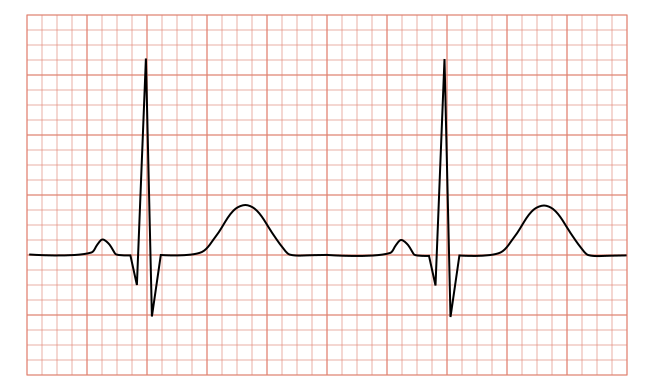
\includegraphics[width=0.5\textwidth]{EKG.png}
\end{figure}

\begin{itemize}
    \item Vad visualiseras i ett EKG? Beskriv vad som sker i hjärtat kortfattat.
    \item Hur kan ett EKG användas för att upptäcka hjärtsjukdomar?
\end{itemize}
\vspace{80mm}

\question \textbf{BONUS}: Beskriv något du lärt dig och tyckt varit extra intressant, men som inte var med på provet! (\textbf{2 bonuspoäng})

\end{questions}

\end{document}
